%%%%%%%%%%%%%%%%%%%%%%%%%%%%%%%%%%%%%%%%%%%%%%%%%%%%%%%%%%%
% --------------------------------------------------------
% Rho
% LaTeX Template
% Version 2.0.0 (21/05/2024)
%
% Authors: 
% Guillermo Jimenez (memo.notess1@gmail.com)
% Eduardo Gracidas (eduardo.gracidas29@gmail.com)
% 
% License:
% Creative Commons CC BY 4.0
% --------------------------------------------------------
%%%%%%%%%%%%%%%%%%%%%%%%%%%%%%%%%%%%%%%%%%%%%%%%%%%%%%%%%%%

\documentclass[11pt,proc,twoside]{RMxAC_rho-class/RMxAC_rho}
\setbool{rho-abstract}{true} % Set false to hide the abstract
\setbool{rho-resumen}{true} % Set false to hide the abstract
\setbool{corres-info}{true} % Set false to hide the corresponding author section
\setbool{linenumbers}{true} % Set false to hide the line numbering

\newcommand\rmaatex{RMxAC}
\newcommand{\CS}[1]{\texttt{\textbackslash #1}}
%----------------------------------------------------------
% volume
%----------------------------------------------------------
\vol{59}
%
\newenvironment{Example}
{\begin{list}{}{\setlength{\leftmargin}{10pt}\setlength{\rightmargin}{10pt}}%
  \item[]\itshape}
  {\end{list}}


%----------------------------------------------------------
% TITLE
%----------------------------------------------------------
%\journalname{\Large Revista Mexicana de Astronomía y Astrofísica 62, 1-10 (2026) \hfill {\includegraphics[width=1.2in, height=0.5in]{LogoRMxACamarillo.png}} \\}

\title{ Extended contribution using the \rmaatex ~ template  v1.0}

%----------------------------------------------------------
% AUTHORS AND AFFILIATIONS
%----------------------------------------------------------

\author[1,$\dagger$]{Irene~Cruz-González \orcidlink{0000-0002-2653-1120}}
\author[2]{Carlos~G.~ Román-Zúñiga \orcidlink{0000-0001-8600-4798}}
\author[3,$\dagger$]{William~J.~Henney \orcidlink{0000-0001-6208-9109}}
%\author[1,2,$\dagger$]{A. Student}
%\author[2,4]{M.~Y.~Posdoc}

%----------------------------------------------------------

\affil[1]{Universidad Nacional Autónoma de México, Instituto de Astronomía, AP 106,  Ensenada 22800, BC, México}
\affil[2]{Universidad Nacional Autónoma de México, Instituto de Radioastronomía y Astrofísica.\\
Antigua Carretera a Pátzcuaro 8701, Ex-Hda. San José de la Huerta, 58089, Morelia, Michoacán, México}
\affil[3]{Universidad Nacional Autónoma de México, Instituto de Astronomía, AP 70-264, CDMX 04510, México}

%\affil[4]{One more affiliation you may need}
%\affil[$\dagger$]{This project is part of a collaboration/consortium/program}


%----------------------------------------------------------
% DATES
%----------------------------------------------------------

%\dates{This manuscript was compiled on June 25th, 2024}

%----------------------------------------------------------
% FOOTER INFORMATION
%----------------------------------------------------------

\leadauthor{Cruz-González et al.}
\smalltitle{{\bf {\it Local Volume Mapper III},
Zihuatanejo, Gro., México, September 10-15 2026.
Editors for this issue: Milky Way, Magellanic Cloud \& Messier 33}}


%\institution{Universidad Nacional Autónoma de México}
%\footinfo{Creative Commons CC BY 4.0}
%\theday{November 20th, 2024} %\today

%----------------------------------------------------------
% ARTICLE INFORMATION
%----------------------------------------------------------

\corres{Irene Cruz-González}
\email{icruzgonzalez@astro.unam.mx}

\received{\today}
%\revised{April 16, 2024}
\accepted{April 20, 2025}
%\published{May 21, 2024}
\doi{\url{https://www.astroscu.unam.mx/rmaa/RMxAA..XX-X}}

%\license{Rho LaTeX Class \ccLogo\ This document is licensed under Creative Commons CC BY 4.0.}

%----------------------------------------------------------
% ABSTRACT
%----------------------------------------------------------

\begin{resumen}
Bienvenidos a los nuevos macros de la \rmaatex\  (v1.0 31/02/2025) para preparar su contribución a las memorias de congresos para ser publicados en la RMxAC. Hay tres tipos de macros de la Serie de Conferencias:  “rm-extenso”, “rm-onepage” or “rm-shortabstract”, dependiendo del caso. Hay una guía complementaria  {\it RMxACauthorguide} que describe los macros en detalle. \\Este es el ejemplo de una contribución en {\it extenso}, para las contribuciones invitadas y/o en extenso.
\end{resumen}

\begin{abstract}
Welcome to the \rmaatex\ template (v1.0 31/02/2025) to prepare your contribution to the proceeding of the conference to be published in RMxAC. There are three types of macros for contributions for publication in the Serie de Conferencias:  “rm-extenso”, “rm-onepage” or “rm-shortabstract”, depending on the case. There is a complementary {\it RMxAA-authorguide} that describes details of the macros. \\{\bf This is the {\it extenso} example, for invited and extended contributions.}
\end{abstract}



%----------------------------------------------------------

\keywords{keyword 1, keyword 2, keyword 3, keyword 4, keyword 5}

\pclave{palabra clave 1, palabra clave 2, palabra clave 3}

%----------------------------------------------------------

\begin{document}
	
\maketitle

%\pagestyle{fancy}
\thispagestyle{firststyle}
%\tableofcontents

%----------------------------------------------------------

\section{Introduction}

There are three types of macros for contributions for publication in the Serie de Conferencias (RMxAC):  “rm-extenso”, “rm-onepage” or “rm-shortabstract”, depending on the case. The style of this template is based on the \textit{rho class} style. It requires minimal or no typesetting adjustments to provide a version of your manuscript organization that will be close to its final printed version. This style also has ample margins to allow for a comfortable number of words per line and to leave room for marginal notes. There is a complimentary author guide with details {\it RMxAA-authorguide}, which requires some familiarity with the use of \LaTeX{} and {\it Overleaf online editor} \url{https://www.overleaf.com}, where the RMxAC macros in \LaTeX{} can be obtained and used. For the author who requires a general introduction to \LaTeX{}, we recommend starting at {\it The LaTeX Project} website \url{https://www.latex-project.org/about/}, or using the Overleaf LaTeX guide\url{https://www.overleaf.com/learn/latex/Free_online_introduction_to_LaTeX_(part_1)}. 

\section{Preamble}

The first line to appear in your document should be 

\bigskip
\CS{documentclass}\verb+{RMxAC_rho}+

\bigskip
or

\bigskip
\CS{documentclass}[\textbf{optionlist}]\verb+{RMxAC_rho}+

\bigskip
\noindent which sets up the document to use the RMxAC class, using the default \texttt{manuscript} option, which is designed for use by authors who submit extended articles to the RMxAC journal. 

The following commands can be used after the \CS{documentclass} command, and before the command \CS{begin}\verb|{document}|: %{\mathrm{document}\}$:

\begin{itemize}
    \item \CS{title} -- defines article title
    \item \CS{author} command defines the authors of the article.
    \item \CS{affil} -- defines the author´s affiliations
    \item \CS{leadauthor} -- provides the last name and initials of the leading author of the article, and will be visible at the top of every odd-number page.
    \item \CS{smalltitle} -- defines the footer that appears at the bottom of the page of every article in RMxAC, and it is used to register the details of the meeting: conference title, city and country, date, and special volume editors.
    \item \CS{corres} and \CS{email} define the name and email address of the corresponding author.
\end{itemize}



\section{Abstract and keywords}

The {\it abstract} and {\it resumen} of the article are placed between the commands: \CS{begin}\verb|{abstract}| ... \CS{end}\verb|{abstract}| and \CS{begin}\verb|{resumen}| ... \CS{end}\verb|{resumen}|. The recommended size for both is 12 lines maximum.

If the authors are unable to provide a Spanish version of the abstract, you can use the same text as for the English abstract, and our editors will take care of the Spanish version.
 

Below the abstract, a minimum of three keywords and a maximum of five keywords must be placed using the command \verb|\keywords{}|. Equivalently, the keywords provided as "palabras clave" in Spanish using the command \verb|\pclave{}| will be taken care of by the editors.

\section{Main Body}

The main body of the document should be enclosed within the following pair of commands:

\bigskip
\CS{begin}\verb+{document}+

...

ARTICLE TEXT

...

\CS{end}\verb+{document}+
\bigskip

The first command after the \CS{begin}\verb+{document}+ should be \CS{maketitle}. This will format title, authors, abstracts, and key words.

Within the main body of the document all standard \LaTeX{} commands can be used. The commands provided by the many optional packages distributed with \LaTeX{} may also be used as long as the package is loaded using the \CS{usepackage} command in the preamble. However, authors are requested to avoid using commands that change document fonts, page layout, or other ``stylistic" parameters. We should also note that not all optional packages have been tested for compatibility with the rmaa\_rho class.

\subsection{Sectioning commands and cross references}

Authors are encouraged to use the standard \LaTeX{} sectioning commands to subdivide their article:

\bigskip

\CS{section}

\CS{subsection}

\CS{subsubsection}

\CS{paragraph}

\bigskip

Please use standard \LaTeX{} sectioning commands to subdivide your document. You should use mixed cases for the section titles, although in the current style this only really matters at the level of \CS{subsection} and below.

These will be automatically typed in the RMxAA and RMxAC style. Cross-referencing is made easier by the use of the \CS{label} 
 \verb+{LABEL}+ command immediately after each sectioning command, where the LABEL text is any mnemonic string. Elsewhere in the document, the section can then be referred to as \S \CS{ref} \verb+{LABEL}+. The \CS{label} command can also be used with equations and with figures and tables (see below). 

It is preferable to use the \CS{label}/\CS{ref} mechanism for cross references in order to minimize the chance of errors and
allow automatic hyperlinks in the PDF output. The style that should be used for cross references is, for example, Figure 3, Table 1, equation (12), and \S 5.1, where the symbol of the section “§” is produced by the \LaTeX{} command “\S”.

\subsection{Math Symbols and Equations}
\label{sec:math}

Symbols for physical quantities should usually be in italics: velocity,
$v$, density, $N$, etc. However, multi-letter symbols generally look
better in roman: FWHM, EM, etc. 

The subscripts should be in roman (coded using \CS{mathrm}) unless they are themselves variables:
$N_\mathrm{e}$, $T_\mathrm{eff}$, but $\sum_i a_i$. 

Physical units should be in roman with thin spaces: $10\,\mathrm{K}$, $1.2\times
10^{-12} \,\mathrm{erg\,cm^{-2}\,s^{-1}}$, etc. 

Things generally come
out best if you place an entire expression within a single pair of\$'s and then make judicious use of \CS{mathrm}. For example,
\begin{Example}
  $ \mathrm{FWHM} = \int N_\mathrm{e} N_\mathrm{i} \, dz $ 
\end{Example}

Recall that the ``minus sign" only exists inside math mode: minus two is $-2$, not~-2, nor \hbox{even --2!} Also, remember that spacing insidemath mode is designed for equations, not words, so you should not use\$'s just to get italic text. Compare $eff$ and \textit{eff}. 

The \CS{frac} command (and its \TeX{} relative \CS{over}) are best only used in the displayed equations. Something like 
\begin{equation}
  \label{eq:one}
  x = \frac { a + b } { c } 
\end{equation}
looks fine, whereas $x = \frac { a + b } { c }$ is somewhat cramped. Better rewritten as $x = (a + b) / c $. 

\paragraph{How to define a macro that can be used inside or outside  math mode.} Use the \CS{ensuremath} command. For example: 
\begin{verbatim}
\newcommand{\fluxunits}{%
   \ensuremath{\mathrm{%
      erg\,s^{-1}\,cm^{-2}}}}
\end{verbatim}
Then you can write either \verb+15.1\,\fluxunits+ or
\verb+$2.3\times+ \verb+10^{-11} \,+ \verb+\fluxunits$+

\subsubsection{Equations}

Equation~\ref{ec:equation}, shows the Schrödinger equation as an example:     \begin{equation} \label{ec:equation}
         \frac{\hbar^2}{2m}\nabla^2\Psi + V(\mathbf{r})\Psi = -i\hbar \frac{\partial\Psi}{\partial t}
    \end{equation} 
Punctuation can be added as in Eq.~\ref{ec:equation3}
    \begin{equation} \label{ec:equation3}
         \frac{\hbar^2}{2m} \nabla^2\Psi + V(\mathbf{r})\Psi = -i\hbar \frac{\partial\Psi}{\partial t}.
    \end{equation} 
    
\subsection{Special symbols}

The commands for commonly used symbols in astronomy are presented in Table~\ref{tab:anysymbols}.

\begin{table}[H]
\caption{Astronomy special symbols commands.}%Additional commands for special symbols commonly used in astronomy. These can be used anywhere.}
 \label{tab:anysymbols}
 \centering
 \begin{tabular*}{0.80\columnwidth}{@{}l@{\hspace*{20pt}}l@{\hspace*{20pt}}l@{}}
  \hline
  Command & Output & Meaning\\
  \hline
  \verb'\sun' & \sun & Sun, solar\\[2pt] % additional height spacing for enhanced symbol legibility
  \verb'\earth' & \earth & Earth, terrestrial\\[2pt]
  \verb'\micron' & \micron & microns\\[2pt]
  \verb'\degr' & \degr & degrees\\[2pt]
  \verb'\arcmin' & \arcmin & arcminutes\\[2pt]
  \verb'\arcsec' & \arcsec & arcseconds\\[2pt]
  \verb'\fdg' & \fdg & fraction of a degree\\[2pt]
  \verb'\farcm' & \farcm & fraction of an arcminute\\[2pt]
  \verb'\farcs' & \farcs & fraction of an arcsecond\\[2pt]
  \verb'\fd' & \fd & fraction of a day\\[2pt]
  \verb'\fh' & \fh & fraction of an hour\\[2pt]
  \verb'\fm' & \fm & fraction of a minute\\[2pt]
  \verb'\fs' & \fs & fraction of a second\\[2pt]
  \verb'\fp' & \fp & fraction of a period\\[2pt]
 % \verb'\diameter' & \diameter & diameter\\[2pt]
  \verb'\sq' & \sq & square, Q.E.D.\\[2pt]
  \hline
 \end{tabular*}
\end{table}


\subsection{Ionization states}

For ions a \verb'\ion{}{}' command is used, for the correct typesetting of ionization states.
For example, to typeset singly ionized calcium, use \verb'\ion{Ca}{ii}', which produces \ion{Ca}{ii}, while a double-ionized forbidden oxigen line produces [\ion{O}{iii}].

\section{Codes}

    This class\footnote{Hello there! I am a footnote :)} includes the \textit{listings} package, which offers customized features for adding codes specially for C, C++, \LaTeX\ and Matlab. You can customize the format in \textit{rho class} file.

    \nolinenumbers
    \lstinputlisting[caption=Example of matlab code., label={lst:listing-Mat}, language=Matlab]{example.m}
    \linenumbers
    
    If line numbering is enabled, we recommend placing the command \verb|\nolinenumbers| at the beginning and \verb|\linenumbers| at the end of the code. 
    
    This will temporarily remove line numbering and the code will look better.
    


\section{Figures and tables}

    \subsection{Sample figure}

        Figure \ref{fig:figure} shows an example figure.
        
            \begin{figure}[ht]
                \centering
                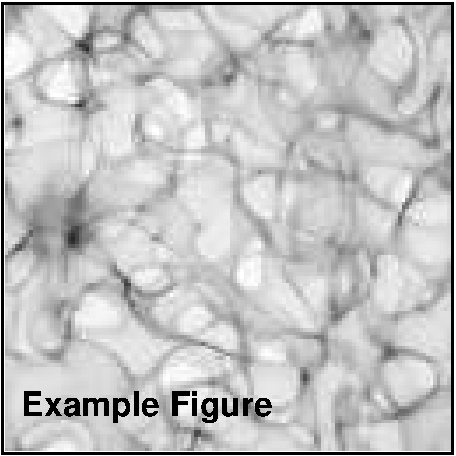
\includegraphics[width=0.75\columnwidth]{figures/example-fig.pdf}
                \caption{Example figure of size = 0.75 columnwith.}
                \label{fig:figure}
            \end{figure}

    \subsection{Sample double figure}

        Figure~\ref{fig:examplefloat} shows an example of a floating figure of two pictures that covers the width of the page. It can be placed at the top or bottom of the page. The space between the figures can also be changed using the \verb|\hspace{Xpt}| command.

        \begin{figure*}[ht] % t for position at the top of the current page; b for position at the bottom of the current page
            \centering
                \begin{subfigure}[b]{0.38\linewidth} % Fig (a)
                    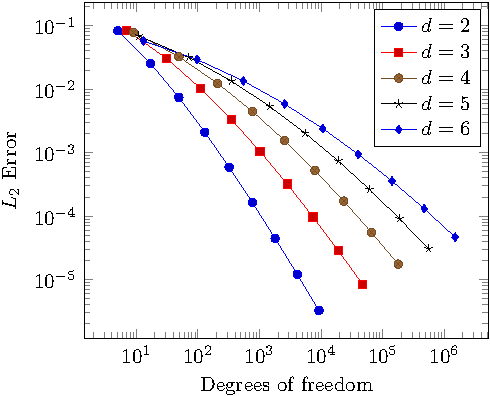
\includegraphics[width=\linewidth]{figures/example2.pdf}
                    \caption{Example left figure.}
                    \label{fig:figa}
                \end{subfigure}
            \hspace{15pt}   % Space between the figures
                \begin{subfigure}[b]{0.38\linewidth} % Fig (b)
                    \centering
                    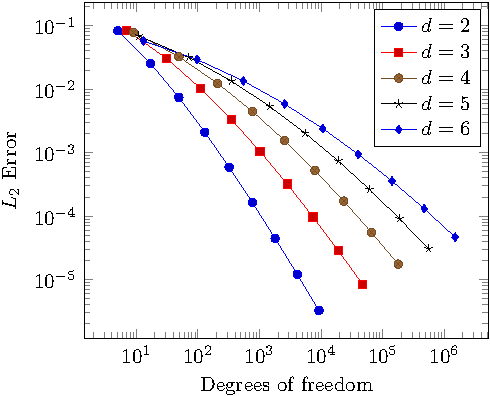
\includegraphics[width=\linewidth]{figures/example2.pdf}
                    \caption{Example right figure.}
                    \label{fig:figb}
                \end{subfigure}
            \caption{Example figure that covers the width of the page obtained from PGFPlots \cite{PFGPlots}.}
            \label{fig:examplefloat}
        \end{figure*}

    \subsection{Sample table}

    In the same way as in the figures, the tables can be placed in one or two columns, depending on the table length.

        Table~\ref{tab:table2}, shows an example table that covers the width of the page positioned at the bottom of a new page. Table~\ref{tab:table2}, shows an example of a column-width table positioned at the top of a page.

        \begin{table*}[ht]
            \RaggedRight
            \caption{Table example that covers the width of the page.}
            \label{tab:table2}
                \begin{tabular}{lllp{11.2cm}}
                    \toprule
                    \textbf{Day} & \textbf{Min Temp} & \textbf{Max Temp} & \textbf{Summary} \\ 
                    \midrule
                    Monday & 11\textdegree C & 22\textdegree C & A clear day with lots of sunshine.  Strong breeze will bring down the temperatures. \\
                    Tuesday & 9\textdegree C & 19\textdegree C & Cloudy with rain, across many northern regions. \\
                    Wednesday & 10\textdegree C & 21\textdegree C & Rain will still linger for the morning. 
                    Conditions will improve by early afternoon and continue 
                    throughout the evening.\\
                    \bottomrule
                \end{tabular}
                
            \tabletext{Note: Obtained from Latex tables \cite{projects-2023}.}
            
        \end{table*}

        
        \begin{table}[ht]
            \RaggedRight
            \caption{Table example that covers one column of the page.}
            \label{tab:table3}
                \begin{tabular}{lccl}
                    \toprule
                    \textbf{Day} & \textbf{$T_{min}$} & \textbf{$T_{max}$} & Reference \\ 
                    \midrule
                    Monday & 11\textdegree C & 22\textdegree C & \citet{1987flme.book.....L}\\
                    Tuesday & 9\textdegree C & 19\textdegree C & \citet{1987flme.book.....L} \\
                    Wednesday & 10\textdegree C & 21\textdegree C & \citet{1987flme.book.....L}\\
                    \bottomrule
                \end{tabular}
                
            \tabletext{Note: Similar a Table~2, de ancho de una columna, con referencia y nota}.
            
        \end{table}

        If the table exceeds the width of the page, the environment \verb'\begin{landscape}' ... \verb'\end{landscape}' can be used. Unfortunately, this method will force a page break before the table appears. Authors should not worry, since this will be corrected in editorial work.

\section{Appendices}

If you have appendices to the article, you can
use something like the following:\\
\CS{begin}\verb|{appendices}|\\
\CS{section}\verb|{First Appendix}|\\
\CS{label}\verb|{sec:ap-A}}|\\
\CS{}\verb|{Text of first appendix.}|\\
\CS{section}\verb|{Second Appendix}|\\
\CS{label}\verb|{sec:ap-B}|\\
\CS{}\verb|{Text of second appendix.}|\\
\CS{end}\verb|{appendices}|\\

The appendices go after the acknowledgments but before the
bibliography. Equations in the appendices will be labeled
A1, A2, B1, B2, etc.

\section{Concept highlight box}

The new \rmaatex macro allows the authors to use a colored box to highlight a concept or an equation, as shown in the example. The label and reference point to the section that it is included in. Example: See the Concept box in Section~\ref{box:box1}.  
    
        \begin{rhoenv}[frametitle=Highlight Concept Box]
            Hello! I am an example of a concept highlight box. \label{box:box1}
        \end{rhoenv}
    


%\section*{Unnumbered section} \label{sec:unsec}

%    If an unnumbered section is declared, a square appears followed by the section name. This style is characteristic of this class and is only for first level sections.

%    Since this affects the title of the table of contents and references, you can make a modification in \textit{section style-rho class} to remove the square. See appendix for more information.

\section{Reference style}

    The default formatting for references follows the Astrophysics Data System (ADS) BibTeX style. The author should provide a bibliography file using the command \CS{bibliography}\verb|{bibfile}| where all references are included. At the end of the document, you will find an example of the default reference formatting. 
    
    The usual commands \CS{citep} for reference in parentheses, as in \citep{Roman23},  and \CS{citet} for references with year in parentheses, as in \citet{Roman23}, are used in the main body of the article.

    %You can modify the style of your references, for that, go to rho-class/rho.cls/biblatex. See the Appendix for more information.

%-------------References bib file------------------------

\bibliography{rmxac}

%----------------------------------------------------------

\end{document}
